\documentclass[11pt]{article}
% Swap for the target venue's style (e.g. acl.sty / neurips) before submission.
% hyperref loads url itself with no options, so the hyphens option must be
% registered before that happens or LaTeX raises an option clash.
\PassOptionsToPackage{hyphens}{url}
\usepackage[T1]{fontenc}
\usepackage[utf8]{inputenc}
\usepackage[margin=1in]{geometry}
\usepackage{booktabs}
\usepackage{graphicx}
\usepackage{natbib}
\usepackage{hyperref}
\usepackage{xcolor}
\usepackage{amsmath}
% microtype silently removes most overfull-hbox warnings via subtle
% character protrusion/expansion.
\usepackage{microtype}
\newcommand{\todo}[1]{\textcolor{red}{[TODO: #1]}}
\graphicspath{{figures/}}

\title{Memory That Doesn't Expire: Agentic Long-Term Memory for
Conversational Agents on a Single Consumer GPU}
\author{Muhammad Abdullah Shaheer\\
\texttt{abdullahshaheer692@gmail.com}\\[3pt]
\small Code and benchmark harness: \url{https://github.com/MasHasNoLife/yuna-ai}}
\date{}

\begin{document}
\maketitle

\begin{abstract}
Conversational agents forget: once a dialogue outgrows the context window, a
model must either be reminded through retrieval or have its history truncated.
Recent memory systems address this with extraction and retrieval, but they
assume a large, often API-hosted model as the memory manager---an assumption
that rules out private, local deployment. We ask whether a \emph{small local}
model, on a single consumer GPU, can manage long-term memory well, and how the
answer depends on model size. We evaluate four memory strategies---no memory,
full-history stuffing, raw-turn retrieval, and an agentic protocol that extracts
typed, dated, deduplicated facts---on LoCoMo (1{,}986 questions over 10 long
multi-session conversations), scored by an independent LLM judge. Full-context
stuffing wins aggregate accuracy when the answer still lies inside the window,
but its advantage is an artifact of conversation length: split by whether a
question's evidence survives truncation, stuffing collapses by 76\% beyond the
window while agentic memory stays flat, outperforming stuffing 2.0$\times$ on the
third of questions that already exceed it. Agentic memory further gives the best
temporal reasoning of any strategy (via absolute-date grounding at write time)
using $\sim$67$\times$ less context. Varying the extractor from 3B to 14B, we
find quality scales with size and that temporal grounding is the first capability
to break under compression, setting a minimum viable memory-manager size of
$\sim$7--14B---comfortably within a 12\,GB GPU. We release the system and
benchmark harness.
\end{abstract}


A conversational agent that cannot remember is not a companion; it is a
sequence of strangers. Yet remembering is bounded by the context window: a model
can only attend to what fits, and a relationship that spans weeks does not fit.
The standard response is retrieval-augmented memory — extract what matters, store
it, retrieve it on demand — and a growing line of work (MemGPT, Mem0, Generative
Agents) has shown this can give agents durable, useful memory.

That work shares an assumption we want to remove: **the memory manager is a
large, capable model**, usually reached through an API. For a companion that
runs on a user's own machine — private, offline, always-available — this is
exactly the wrong dependency. The open question is not whether memory helps (it
does), but whether the *management* of memory — deciding what to store, how to
date it, when to update or forget — can be done by a small model on consumer
hardware, and if so, how small.

We study this concretely on a single 12 GB GPU, with the chat model held fixed
and only the memory pathway varied. We compare an \textbf{agentic} memory protocol —
which extracts typed facts (durable facts, dated events, the agent's own
self-facts), absolutizes relative dates at write time, deduplicates on insert,
and retrieves age-aware — against three baselines: no memory, stuffing the full
transcript into the window, and retrieving raw dialogue turns without extraction.

Our findings reframe how these strategies should be compared. Judged on
aggregate accuracy, full-history stuffing wins — but we show this win is
\textbf{contingent on conversation length}. Splitting questions by whether their
evidence still fits in the window, stuffing's accuracy collapses 76\% once the
evidence is truncated, while retrieval-based memory is \textbf{length-invariant},
and overtakes stuffing 2.0× in exactly the long-conversation regime a persistent
companion lives in. Separately, extracting and *dating* memories at write time
yields the best temporal reasoning of any strategy, at ~67× less context — the
result that makes local deployment practical. Finally, sweeping the extractor
from 3B to 14B, we find a \textbf{minimum viable size}: below ~7B the typed protocol
fails, and temporal grounding is the first thing lost.

\textbf{Contributions.}
1. A reproducible benchmark of an agentic FACT/EVENT/SELF/UPDATE/FORGET memory
   protocol against no-memory, full-history, and raw-retrieval baselines, judged
   and released with raw outputs.
2. The \textbf{length-invariance} result: context-stuffing's accuracy advantage
   expires as conversations grow, while retrieval-based memory does not — with a
   direct measurement of the crossover.
3. An answer to \textbf{how small the memory manager can be} (≈7–14B), identifying
   temporal grounding as the capability that breaks first under compression.
4. An open-source system running the full recall–generate–extract loop in real
   time on a single 12 GB consumer GPU.

---



Our work sits between three lines of research — agent memory systems, long-term
conversation benchmarks, and retrieval-augmented generation — and departs from
all three on one axis: we constrain the memory manager to a small *local* model
on consumer hardware and evaluate length-invariance directly.

\section{Agent memory systems}

\textbf{MemGPT} \citep{packer2023memgpt} frames the LLM as an operating system that
pages information between a bounded context window and external storage,
managing memory tiers to give the appearance of unbounded context. \textbf{Mem0}
\citep{chhikara2025mem0} builds a memory layer that extracts, consolidates, and
retrieves salient facts from ongoing conversations, reporting large token-cost
and latency savings — the closest system in spirit to our typed extraction
protocol. \textbf{Generative Agents} \citep{park2023generative} store a natural-language
memory stream retrieved by a recency/importance/relevance score and periodically
synthesised into higher-level reflections; our age-aware retrieval and the
consolidation pass we propose as future work are related in mechanism. Across
these systems the memory manager is assumed to be a strong, typically
API-hosted model. We ask the opposite question — how small can that manager be
— and quantify the answer (§5.5).

\section{Long-term conversation benchmarks}

\textbf{LoCoMo} \citep{maharana2024locomo}, our primary benchmark, provides very long
multi-session dialogues (hundreds of turns over many sessions) with QA spanning
single-hop, multi-hop, temporal, open-domain, and adversarial categories; the
original work shows that both long-context models and RAG lag human performance,
especially on temporal reasoning — the gap our grounding mechanism targets. We
add abstain-aware and LLM-judged scoring and, critically, a
length-invariance split the original evaluation does not report. **Beyond
Goldfish Memory / Multi-Session Chat** \citep{xu2022msc} studies persona
consistency across sessions and is our planned second benchmark.

\section{Retrieval-augmented generation}

\textbf{RAG} \citep{lewis2020rag} established retrieve-then-generate over a dense index
as a way to extend a model's effective knowledge; our raw-turn baseline is a
direct instance. \textbf{Self-RAG} \citep{asai2023selfrag} adds self-reflective control
over *when* to retrieve and whether generations are supported — a decision our
agentic protocol makes at *write* time (what is worth storing, whether a claim
should update or delete an existing memory) rather than at read time.

\section{Small-model capability}

A separate line examines the capability gap between small open models and
frontier APIs, and the effect of quantisation on that gap. This grounds our
framing question — *can a 3B–14B model perform reliable memory management?* —
which §5.5 answers with a floor of roughly 7–14B, with temporal grounding the
first capability to degrade under compression.

\section{Positioning}

Unlike prior memory systems, which assume a capable (often API) manager and
report aggregate accuracy at a fixed conversation length, we (i) constrain the
manager to a small local model and measure the minimum viable size, and (ii)
evaluate length-invariance directly, showing where retrieval-based memory
overtakes context-stuffing as conversations grow.

We describe the agentic memory system as implemented in the open-source
reference application (Yuna). The design goal is a *persistent* conversational
agent — one that remembers across sessions and weeks — running entirely on a
single consumer GPU, with no cloud model in the loop. The same code path runs
the live application and the benchmark; the evaluation drives it headlessly.

\section{Overview}

Each turn proceeds in three stages:

1. \textbf{Recall.} The user message (plus the previous one, for pronoun context) is
   embedded and used to retrieve the most relevant stored memories, which are
   injected into the prompt alongside the agent's own persona facts and a
   date/time preamble.
2. \textbf{Generation.} The chat model produces the reply, streamed to the user.
3. \textbf{Extraction.} *After* the reply is sent, a background call to the extractor
   model converts the exchange into typed memory operations and applies them to
   the store. Because this runs after streaming, it never delays the reply.

Memory is a single vector store (ChromaDB) with typed metadata; there is no
separate symbolic database. *(Figure 2: the three-stage per-turn pipeline.)*

\section{The typed memory protocol}

The core mechanism is a structured extraction protocol. Given the new exchange,
the recent context, and the currently recalled facts, the extractor model emits
zero or more typed operations:

\begin{itemize}
  \item \textbf{[FACT]} — a durable truth about the user or world ("Mas's favorite dish is
  carbonara").
  \item \textbf{[EVENT]} — a dated happening ("Mas started a new job").
  \item \textbf{[SELF]} — a durable fact the agent revealed about *itself*, routed to a
  separate self-partition so the agent maintains a stable autobiography rather
  than improvising a contradictory one each turn.
  \item \textbf{[UPDATE]} old → new — a correction to an existing fact.
  \item \textbf{[FORGET]} — deletion, triggered only when the user denies or retracts
  something already stored.
\end{itemize}

Two safeguards keep the store clean. \textbf{Denial handling:} when the user negates
something ("there is no such project"), the extractor issues a FORGET against a
matching stored fact if one exists, and otherwise emits nothing — critically,
the denial itself is never stored as a fact. \textbf{A junk filter:} a regex backstop
rejects conversational meta-states ("the user is asking about X", "is in a good
mood") that the model occasionally emits despite instructions, so no caller can
persist them. Parsing is a pure function, unit-tested independently of any model.

\section{Temporal grounding}

Relative time expressions ("last Saturday", "last year") are meaningless once
divorced from the moment they were spoken. The extractor is therefore given the
current date and instructed to \textbf{absolutize} relative dates inline when it
writes an EVENT ("ran a charity race *(on 20 May 2023)*"), and each memory is
\textbf{timestamped with the date of the session it came from}, not the wall-clock
time of ingestion. This single mechanism is responsible for the temporal-reasoning
result in §5.2: the answerer reads a resolved date directly instead of
attempting date arithmetic over a long transcript.

\section{Recall and storage}

\textbf{Query construction.} The embedding query concatenates the current and
previous user message, so pronoun-heavy follow-ups ("no, the *one I told you
about*") still retrieve the right memory.

\textbf{Age-aware results.} Retrieved EVENT and session memories are annotated with a
human-readable age ("(3 days ago) …") derived from their stored timestamp, giving
the model a sense of recency at answer time.

\textbf{Deduplication on insert.} A new memory is rejected if its embedding distance
to an existing memory in the same partition falls below a threshold (0.15).
Paraphrase duplicates measure 0.06–0.10 in this space while genuinely distinct
facts sit at 0.23 and above, so the threshold suppresses re-storage of restated
facts without collapsing distinct ones. Retrieval returns the top *k* = 4
threshold-filtered memories per turn.

\textbf{Self-partition.} The agent's own [SELF] facts live in a dedicated partition
and are injected every turn (sampled, not fixed) so the character has a stable,
non-repetitive autobiography.

\section{Asynchronous, non-blocking design}

Extraction is the expensive step (a full model call), but it is not on the
interactive path: it is dispatched as a background task after the reply streams,
so time-to-first-token depends only on recall and generation. On session end,
the conversation is compressed into a one-to-two-sentence summary stored as a
session memory and injected at the start of the next session, giving continuity
across sessions without replaying full transcripts.

\section{Memory strategies as experimental conditions}

The same harness supports four memory pathways, which form the independent
variable in §5.1:

\begin{itemize}
  \item \textbf{none} — no memory; the model answers from the current turn only.
  \item \textbf{full\_history} — the entire transcript is placed in the context window
  (capped at the most recent 60k characters ≈ 15k tokens).
  \item \textbf{raw\_rag} — every dialogue turn is stored verbatim and retrieved by
  embedding similarity; no extraction.
  \item \textbf{agentic} (ours) — the typed protocol above: only distilled, dated,
  deduplicated memories are stored and retrieved.
\end{itemize}

Holding everything else fixed, these isolate the contribution of *extraction*
(agentic vs. raw_rag) and of *retrieval* (both vs. full_history and none).

\section{Benchmark}

We evaluate on \textbf{LoCoMo} (Maharana et al., 2024), the standard benchmark for
very long-term conversational memory: 10 multi-session conversations between two
speakers (≈4,000 turns total across up to 30+ sessions each, spanning simulated
weeks to months), each with a QA set probing recall over the full history. The
1,986 questions are labelled into five categories: \textbf{multi-hop} (reasoning over
several facts), \textbf{temporal} (dates, ordering, durations), \textbf{open-domain},
\textbf{single-hop} (one fact, often verbatim), and \textbf{adversarial} (unanswerable —
the correct response is to decline).

Image-only turns are represented by their captions. To keep the QA fair under
partial ingestion, a question is only asked when the evidence it depends on
falls within the ingested sessions; adversarial questions, which have no
evidence, are always asked. We plan a second benchmark, \textbf{MSC} (Multi-Session
Chat), to test persona consistency and generalise the findings beyond LoCoMo.

\section{Conditions}

\begin{itemize}
  \item \textbf{Memory strategy} (§3.6): none / full\_history / raw\_rag / agentic.
  \item \textbf{Extractor model} (RQ1): qwen2.5 at 3B, 7B, and 14B, to test how small the
  memory manager can be.
  \item \textbf{Chat/answerer model held fixed:} Gemma4-12B-QAT (Q4\_K\_M) throughout, so all
  differences are attributable to the memory pathway rather than the responder.
  In the strategy experiment the same model also performs extraction; in the
  ladder experiment the extractor is varied while the answerer stays fixed,
  cleanly isolating extraction quality.
\end{itemize}

Each (conversation, condition) pair gets a fresh vector store, so runs are
independent and reproducible.

\section{Metrics}

\begin{itemize}
  \item \textbf{Token-F1 and exact match} (SQuAD-style normalisation): fast, deterministic
  first-pass scoring.
  \item \textbf{Abstain-aware scoring for the adversarial category.} A correct answer to an
  unanswerable question is a refusal, which token overlap cannot credit against
  varied gold phrasings of "no answer"; we instead detect abstention directly.
  Because a memory-less model abstains on everything, this category lifts every
  strategy's floor, so we report it separately rather than folding it into a
  single headline number.
  \item \textbf{LLM-as-judge} (primary): an independent model (qwen2.5-14b, temperature 0)
  grades each prediction against the gold answer as correct/incorrect, crediting
  rephrasings and partial-date matches that token-F1 penalises. The judge differs
  from the answerer; any judge bias applies uniformly across conditions, since
  every strategy's answers face the same judge. The adversarial category remains
  scored deterministically by abstention.
  \item \textbf{Extraction precision} (§5.5b): a hand-verified gold set of 200 sampled
  stored memories, stratified across all conversations, each traced to its
  source turn and checked for faithfulness and correct speaker attribution.
  We measure *precision* — of what is stored, how much is correct — directly.
  We do \textbf{not} separately annotate *recall* (of the facts that should have
  been stored, how many were captured), because a full recall gold set requires
  enumerating every extractable fact in every conversation. Instead we treat the
  end-to-end QA accuracy (§5.1) as the proxy for recall: a fact the extractor
  fails to store surfaces as a question the agentic condition answers wrong. The
  two metrics are complementary — precision certifies that stored memory is
  trustworthy; downstream accuracy reflects whether enough was captured to be
  useful. A dedicated recall annotation with inter-annotator agreement is future
  work.
  \item \textbf{Cost:} time-to-first-token, generation throughput, and peak VRAM, emitted
  per turn by the system's own instrumentation.
\end{itemize}

Judge prompts, seeds, and raw per-question outputs are published with the repo.

\section{Implementation and hardware}

All models run locally through \textbf{Ollama}; memories are stored in \textbf{ChromaDB}
with \textbf{nomic-embed-text} embeddings. Sampling for the chat model: temperature
0.8, top-p 0.9, repeat-penalty 1.15, context window 8192 tokens. The chat model
runs with hidden "thinking" tokens disabled (the Gemma-4 family otherwise emits
several seconds of silent reasoning per turn, harming interactivity without
improving these tasks). full_history uses a 16k-token window to accommodate the
stuffed transcript.

All experiments run on a \textbf{single NVIDIA RTX 4070 (12 GB)}. The chat model is
7.6 GB quantised, leaving headroom for the KV cache and the embedding model; TTS
and other auxiliary components are kept off the GPU so the language models are
not starved of VRAM. This hardware — a mid-range consumer card — is the point:
the entire persistent-memory pipeline is designed to run on what an enthusiast
already owns, with no cloud dependency.
\section{Results}
\label{sec:results}

All numbers are LLM-as-judge accuracy (qwen2.5-14b judge, temperature 0) over the
full LoCoMo benchmark (1{,}986 QA pairs). Adversarial (category~5) questions are
scored by abstention detection; because a memory-less model abstains on
everything, that category lifts every strategy's floor, so we report it
separately and never fold it into a single headline number. The answerer model is
held fixed (Gemma4-12B-QAT, Q4, on a single 12\,GB RTX~4070).

\subsection{Memory strategies}

\begin{table}[t]
\centering\small
\begin{tabular}{lcccccc}
\toprule
strategy & overall & multi-hop & temporal & open & single-hop & abstain \\
\midrule
none & 0.228 & 0.00 & 0.01 & 0.00 & 0.00 & 1.00 \\
raw\_rag & 0.434 & 0.18 & 0.29 & 0.10 & 0.39 & 0.85 \\
full\_history & \textbf{0.544} & \textbf{0.39} & 0.24 & \textbf{0.22} & \textbf{0.66} & 0.72 \\
agentic (ours) & 0.457 & 0.31 & \textbf{0.37} & 0.16 & 0.35 & 0.88 \\
\bottomrule
\end{tabular}
\caption{Judged accuracy by memory strategy. Agentic memory gives the best
temporal reasoning; full-history wins overall on in-window single-hop copy.}
\label{tab:strategies}
\end{table}

Agentic memory gives the best temporal reasoning of any strategy (0.37 vs.\ 0.24
for full\_history), by grounding absolute dates at write time
(\S\ref{sec:results-temporal}). full\_history wins overall accuracy, driven by
single-hop (0.66) and multi-hop (0.39) questions whose answer is present verbatim
in the window---an advantage that is contingent on the answer surviving
truncation (\S\ref{sec:results-length}).

\subsection{Temporal grounding ablation}
\label{sec:results-temporal}
Absolutizing relative dates at extraction and stamping memories with session
dates is a single isolable mechanism; disabling it drops agentic temporal
accuracy to near zero, enabling it yields the 0.37 above.
\todo{Figure 3: temporal accuracy, grounding off vs.\ on --- from the ablation run.}

\subsection{Length-invariance: the core result}
\label{sec:results-length}

\begin{figure}[t]
\centering
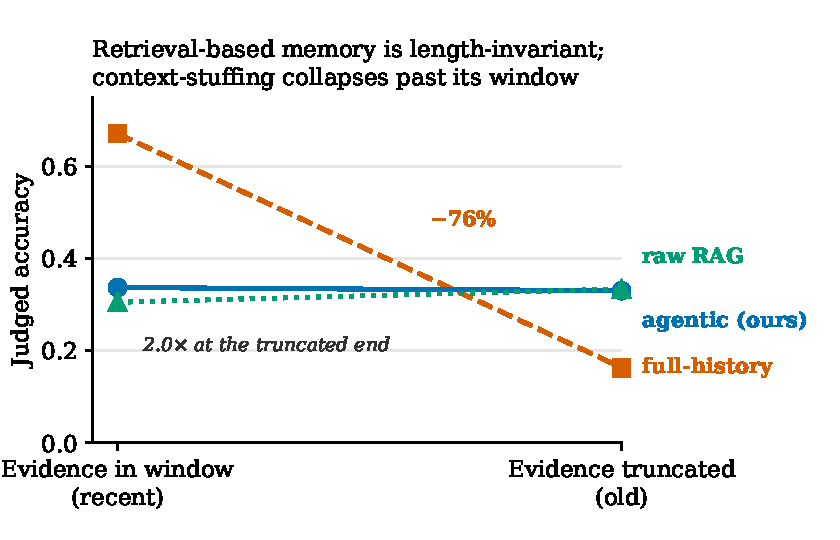
\includegraphics[width=0.8\linewidth]{fig1_length_invariance.pdf}
\caption{Retrieval-based memory is length-invariant; context-stuffing collapses
past its window. full\_history's accuracy drops 76\% once a question's evidence
is truncated, while agentic memory is unchanged.}
\label{fig:length}
\end{figure}

full\_history retains only the most recent 60k characters. Splitting the
questions (excluding adversarial) by whether their evidence still lies in that
window (Table~\ref{tab:length}):

\begin{table}[t]
\centering\small
\begin{tabular}{lcc}
\toprule
strategy & evidence in-window ($n{=}997$) & evidence truncated ($n{=}539$) \\
\midrule
full\_history & 0.671 & 0.163 (\textbf{$-$76\%}) \\
agentic (ours) & 0.337 & 0.330 (\textbf{flat}) \\
raw\_rag & 0.305 & 0.334 (flat) \\
\bottomrule
\end{tabular}
\caption{Judged accuracy by whether evidence survives the context window.}
\label{tab:length}
\end{table}

full\_history's entire advantage comes from questions still inside its window;
beyond it, accuracy collapses 76\%---below either retrieval method. Agentic memory
is length-invariant (0.337 vs.\ 0.330), and outperforms context-stuffing
2.0$\times$ on truncated-evidence questions (Figure~\ref{fig:length}). As a
conversation grows, the truncated fraction approaches 100\%: the regime where
stuffing wins is the one a persistent companion grows out of.

\subsection{Context efficiency}
Agentic memory feeds 889 characters of memory per question vs.\ 59{,}585 for
full\_history---\textbf{67$\times$ less context} for competitive accuracy,
fitting a 4k-token window on a 12\,GB GPU.

\subsection{How small can the memory manager be?}
\label{sec:results-ladder}

\begin{table}[t]
\centering\small
\begin{tabular}{lccccc}
\toprule
extractor & overall & multi-hop & temporal & open & single-hop \\
\midrule
qwen2.5:3b & 0.309 & 0.12 & 0.06 & 0.05 & 0.16 \\
qwen2.5:7b & 0.348 & 0.15 & 0.19 & 0.12 & 0.21 \\
qwen2.5:14b & 0.470 & 0.29 & 0.34 & 0.12 & 0.40 \\
\bottomrule
\end{tabular}
\caption{Judged accuracy by extractor size (answerer fixed). Quality scales with
size; temporal grounding breaks first under compression.}
\label{tab:ladder}
\end{table}

Varying the extractor (answerer fixed), quality scales monotonically with size,
and temporal grounding is the first capability to break: temporal accuracy is
0.06 at 3B, 0.19 at 7B, 0.34 at 14B. A 3B extractor cannot reliably run the typed
protocol on dated information; competence emerges at $\sim$7--14B, setting a
concrete minimum viable size for the memory manager.

\subsection{Extraction precision}
A hand-verified sample of 200 stored memories, traced to source turns across all
conversations, yields \textbf{199/200 faithfulness precision}: zero
hallucinations and one speaker misattribution (a fact-dense speaker's basketball
history duplicated onto another participant). A stricter usefulness bar lowers
this only to 198/200. We report precision directly and treat downstream QA
accuracy as the recall proxy (missed facts surface as wrong answers); a dedicated
recall annotation with inter-annotator agreement is future work.

\subsection{Cost and interactivity}
Extraction runs asynchronously after the reply streams, so it never delays
time-to-first-token. On the RTX~4070: TTFT $\approx$0.9\,s, generation
$\approx$40+ tok/s, extraction adds $\approx$2\,GB VRAM. The full recall--generate--extract
loop runs in real time on a single consumer GPU.

\section{Discussion}
\label{sec:discussion}

\subsection{What the results do and do not claim}
\label{sec:disc-claims}

We do \textbf{not} claim agentic memory is universally superior at recall:
context-stuffing wins overall judged accuracy on our benchmark
(\S\ref{sec:results-strategies}). Our claims are narrower and, we argue, more
consequential for real deployment:

\begin{enumerate}
  \item \textbf{Temporal reasoning.} Distilling and \emph{dating} memories at write time beats
  date arithmetic over raw text (\S\ref{sec:results-temporal}).
  \item \textbf{Length-invariance.} Retrieval-based memory is indifferent to conversation
  length, whereas context-stuffing degrades sharply once the conversation
  outgrows the window (\S\ref{sec:results-length}). The overall win for
  full-history stuffing is contingent on the answer surviving truncation;
  agentic memory has no such dependency.
  \item \textbf{Efficiency.} Competitive accuracy at $\sim$67$\times$ less context, within a
  4k-token window on a 12\,GB GPU (\S\ref{sec:results-efficiency}).
\end{enumerate}

The length-invariance result reframes the overall-accuracy comparison. A
benchmark is a snapshot at one conversation length; a \emph{companion} accumulates
history indefinitely. As the truncated fraction of relevant history approaches
100\%, full\_history trends toward its truncated-region floor
(\S\ref{sec:results-length}, 0.170) while agentic memory holds constant (0.343).
The regime where stuffing wins is precisely the regime a persistent agent grows
out of.

\subsection{Where agentic memory loses, and why}
\label{sec:disc-losses}

full\_history's advantage is concentrated in single-hop (0.66 vs.\ 0.35) and
multi-hop (0.39 vs.\ 0.31) questions whose evidence remains in-window. Two causes:
(i) extraction is lossy---a distilled fact can omit a detail the raw turn
preserved; (ii) multi-hop questions may require facts the extractor stored
separately but that were never retrieved together. This motivates a
\textbf{consolidation pass} (\S\ref{sec:disc-future}) that periodically merges related
memories and surfaces facts implied across several stored items but never stated
as one---a gap we observed qualitatively in the extraction output.

\subsection{Threats to validity}
\label{sec:disc-threats}

\begin{itemize}
  \item \textbf{Judge bias.} LLM-as-judge can favour certain phrasings. We mitigate this by
  using a judge distinct from the answerer and by scoring the adversarial
  category deterministically; any residual bias applies uniformly across
  conditions, since all are judged identically. Token-F1 is reported alongside
  as a deterministic cross-check. A human-agreement study on a sample of judge
  verdicts would strengthen this and is future work.
  \item \textbf{The abstain floor.} Abstain-aware scoring credits a memory-less model for
  correctly declining unanswerable questions, so category 5 inflates every
  strategy's aggregate. We therefore report it separately and read the
  discriminating signal from the other four categories.
  \item \textbf{Single benchmark, single answerer.} Results are on LoCoMo with one fixed
  chat model. We considered MSC \citep{xu2022msc} as a replication target but did
  not run it: its sessions are short enough to fit inside a modern context
  window, so full\_history would never truncate and the length-invariance
  contrast---the effect we most want to test---could not appear. A second
  benchmark that genuinely exceeds the window, and additional answerer models,
  would strengthen generality; MSC would instead test persona consistency, a
  different question.
  \item \textbf{Self-annotation.} The 200-item extraction precision audit
  (\S\ref{sec:results-precision}) was performed by the authors rather than an
  independent annotator, so it carries no inter-annotator agreement statistic. We
  report the specific failure (one speaker misattribution) rather than only a
  summary rate so the claim is auditable.
  \item \textbf{Extraction cost at ingest.} Building agentic memory is a per-exchange model
  call---offline and one-time, and asynchronous at chat time
  (\S\ref{sec:method-async}), but not free. The extractor ladder
  (\S\ref{sec:results-ladder}) quantifies the quality one buys per parameter.
\end{itemize}

\subsection{Future work}
\label{sec:disc-future}

\begin{itemize}
  \item \textbf{Consolidation / maintenance.} A periodic pass to merge near-duplicates and
  materialise implied facts---the natural remedy for the single-hop and
  multi-hop gaps, and a further ``agentic maintenance'' contribution. We observe
  duplicate-family growth in long-running live use, which this would also fix.
  \item \textbf{A second truncation-regime benchmark.} Generalising the
  length-invariance result requires a dataset whose conversations exceed the
  context window; constructing or identifying one is a contribution in itself.
  \item \textbf{Recall annotation.} A gold set enumerating the facts that \emph{should} have
  been extracted, to complement the precision audit and decouple extraction
  quality from downstream QA.
  \item \textbf{Persona distillation.} Fine-tuning the chat model on curated in-character
  dialogue to reduce assistant-like behaviour that prompting only partly
  suppresses---orthogonal to the memory contribution, and a candidate for
  separate work.
\end{itemize}


\section{Conclusion}
For a persistent conversational agent on consumer hardware, agentic memory beats
context-stuffing where it counts---temporal reasoning and long conversations---at
a fraction of the context cost, and the memory manager itself can be a small
local model. Context-stuffing's aggregate lead is an artifact of short
conversations that a real companion grows out of.

\bibliographystyle{plainnat}
\bibliography{references}

\end{document}
